% coding:utf-8

%----------------------------------------
%FOSAMATH, a LaTeX-Code for a mathematical summary for basic analysis
%Copyright (C) 2013, Daniel Winz, Ervin Mazlagic, Adrian Imboden, Philipp Langer

%This program is free software; you can redistribute it and/or
%modify it under the terms of the GNU General Public License
%as published by the Free Software Foundation; either version 2
%of the License, or (at your option) any later version.

%This program is distributed in the hope that it will be useful,
%but WITHOUT ANY WARRANTY; without even the implied warranty of
%MERCHANTABILITY or FITNESS FOR A PARTICULAR PURPOSE.  See the
%GNU General Public License for more details.
%----------------------------------------

% coding:utf-8
\documentclass[a4paper,10pt,fleqn]{article}

\usepackage{tech_ber_ei_layout}

\title{Technischer Bericht Schere}

\author{Daniel Winz}
\date{\today~\dtc}


\begin{document}

\maketitle

% \include{about}

\tableofcontents
\newpage

% % coding:utf-8

% coding:utf-8

\section{Basic Clock Modul +}

\subsection{Übersicht}
\begin{frame}
    \frametitle{}
    \framesubtitle{}
      \begin{figure}
        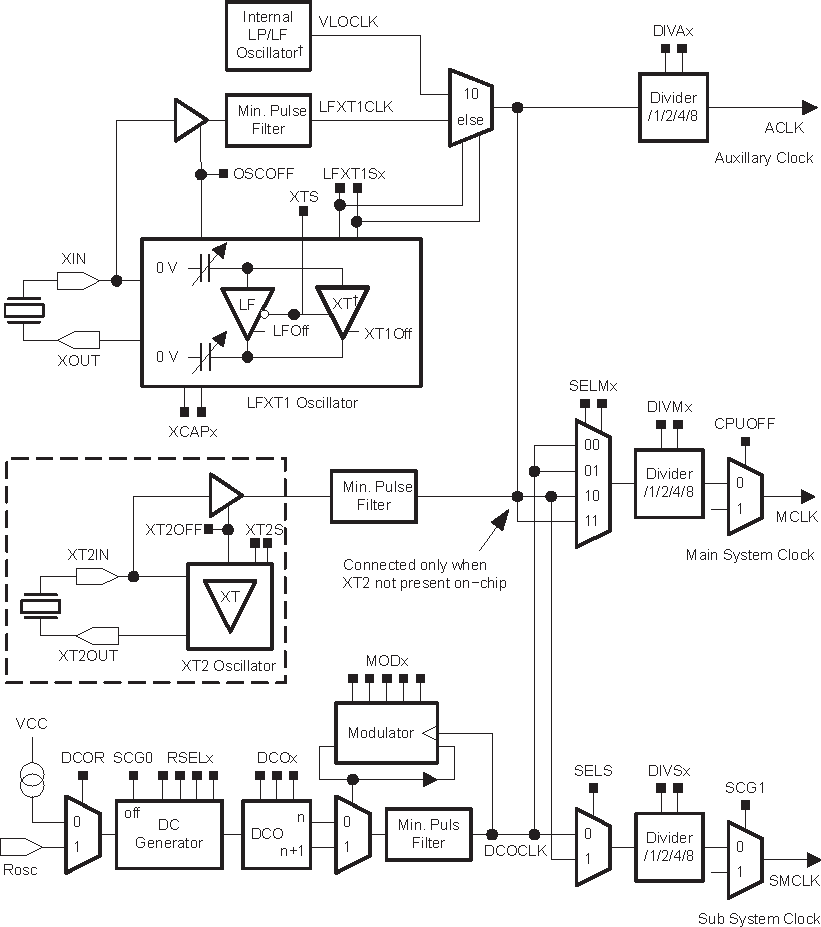
\includegraphics[width=0.5\columnwidth]{fig/ti_fg_bcm_block.pdf}
        \caption{Blockschaltbild}
      \end{figure}

\end{frame}                             % Basic Clock Module
% coding:utf-8

\section{Digitally-Controlled Oscillator}

\subsection{Übersicht}
\begin{frame}
  \begin{center}
\tikzstyle{block} = [ draw,fill=blue!20,text width=5em,align=center,
                      rounded corners,minimum height=3em]
\begin{tikzpicture}
  \uncover<1->{\node[block] at (0,0) (iq) {Stromquelle};}
  \uncover<2->{\node[block] at (3,0) (osc) {RC Oszillator};}
  \uncover<3->{\node[block] at (6,0) (mod)   {Modulator};}
  \uncover<4->{\node at (0,2) (rselx)   {RSELx};}
  \uncover<5->{\node at (3,2) (dcox)   {DCOx};}
  \uncover<6->{\node at (6,2) (modx)   {MODx};}
  \uncover<1->{\draw[-latex] (iq.east) -- (osc.west);}
  \uncover<2->{\draw[-latex] (osc.east) -- (mod.west);}
  \uncover<3->{\draw[-latex] (mod.east) -- ++(right:1);}
  \uncover<4->{\draw[-latex] (rselx.south) -- (iq.north);}
  \uncover<5->{\draw[-latex] (dcox.south) -- (osc.north);}
  \uncover<6->{\draw[-latex] (modx.south) -- (mod.north);}
  \uncover<6->{\draw[-latex] (mod) .. controls (4.7,1) and (4.3,1) .. (osc);}
\end{tikzpicture}
\end{center}

\end{frame}

\subsection{Modulation}
\begin{frame}
  \begin{tikztimingtable}
    \mbox{\uncover<1->{MOD =  0}} & <1->33L<*>\\
    \mbox{\uncover<2->{MOD =  1}} & <2->16LH16L<*>\\
    \mbox{\uncover<3->{MOD =  2}} & <3->8LH15LH8L<*>\\
    \mbox{\uncover<3->{MOD =  3}} & <3->8L2{H7L}H8L<*>\\
    \mbox{\uncover<4->{MOD = 16}} & <4->L16{HL}<*>\\
    \mbox{\uncover<4->{MOD = 24}} & <4->L8{3HL}<*>\\
    \mbox{\uncover<4->{MOD = 31}} & <4->L31HL<*>\\
  \end{tikztimingtable}
\end{frame}

\subsection{Kalibrierung}
\begin{frame}
  \begin{figure}
    
\includegraphics[width=1.0\columnwidth]{fig/ti_ds_dco_freq.pdf}
    \caption{Auszug aus dem Datenblatt des MSP430G2553}
  \end{figure}
\end{frame}
\begin{frame}
  \begin{itemize}
    \item Texas Instruments \pause \\
      MSP430F2x $\rightarrow \pm 1 \%$ \pause \\
    \item Inbetriebnahme \pause
    \item FLL
  \end{itemize}
\end{frame}                             % Digitally-Controlled Oscillator

% \section{Basic Clock Module +}
% \subsection{Übersicht}
% \begin{frame}
%   \frametitle{Ft}
%   \begin{block}{Bt}
%     Funktionsweise des DCO
%   \end{block}
% \end{frame}
\section{Ausgangslage}
Am 15. März 2013 erhalten die Teilnehmer des Moduls Kontext 2 aus dem Bereich 
Elektrotechnik die Aufgabe, eine Vorichtung zu entwickeln, die ein Ei beim Fall 
aus einer Höhe von eineinhalb Metern schützt. Zudem muss das Ei, falls es an 
obiger Vorrichtung befestigt wird, innert nützlicher Frist aus der Vorrichtung 
herausgelöst werden können. Als Material stehen jeder Gruppe 30 Trinkhalme und 
eine Rolle Klebeband zur Verfügung. 
\cite{barmet:aufgabenstellung}

\section{Konzept}
\subsection{Trichter}
Das erste Konzept der Gruppe zwei sieht vor, dass das Ei von einem am Boden 
stehenden Trichter aufgefangen wird. Dieser Trichter soll aus Trinkhalmen 
aufgebaut werden. Dazu werden die Trinkhalme am Gelenk mittels Klebeband an 
ihrem Gelenk zusammengebunden. die langen Enden werden dabei zu einem Trichter 
aufgefächert. Die kurzen Enden werden abgespreizt und dienen somit als 
Standfuss. 

\subsubsection*{Vorteile}
\begin{itemize}
  \item Die Schutzwirkung ist unabhängig davon, in welcher Lage das Ei am Boden 
        ankommt. 
  \item einfacher Aufbau
\end{itemize}

\subsubsection*{Nachteile}
\begin{itemize}
  \item Die Schutzwirkung ist abhängig davon, ob der Trichter getroffen wird. 
  \item Befestigung des Trichters am Boden könnte problematisch sein. 
\end{itemize}

\subsection{"'Airbag"'}
Das zweite Konzept sieht vor, dass das Ei in der Schutzvorrichtung befestigt 
wird. Dazu werden zwei Trichter wie beim vorhergehenden Konzept hergestellt. 
Das Ei wird zwischen den Trichtern Platziert. Anschliessend werden die 
Trichter ineinander geschoben. 

\subsubsection*{Vorteile}
\begin{itemize}
  \item Die Schutzwirkung ist nicht davon abhängig, ob die Schutzvorrichtung 
        getroffen wird. 
  \item Muss nicht am Boden befestigt werden. 
\end{itemize}

\subsubsection*{Nachteile}
\begin{itemize}
  \item Die Lage beim Aufprall ist nicht unerheblich für die Schutzwirkung. 
  \item Der Aufbau ist leicht komplexer als bei einem sich am Boden 
        befindlichen Trichter. 
\end{itemize}

\subsection{Variantenentscheid}
Für die Auswahl eines der obigen Konzepte werden die Vor- und Nachteile der 
beiden Varianten gegeneinander abgewogen. 
Die Komplexität der beiden Varianten unterscheidet sich nur gering. Auch die 
Befestigung von Variante 1 am Boden stellt kein unüberwindbares Hindernis dar. 
Das Risiko, bei Variante 1 den Trichter nicht zu treffen, wird als relativ 
gross eingeschätzt. Die Lage des Eis beim Aufprall wird als beherrschbarer 
betrachtet, als das Treffen des Trichters. 
Der Entscheid fällt aufgrund der obigen Überlegungen zugunsten von Variante 2. 

\subsection{Ausarbeitung des Konzepts}
\begin{figure}[h!]
  \centering
  \includegraphics[width=0.3\columnwidth,clip=true,trim=80mm 250mm 20mm 5mm]
                  {fig/2013-03-15_145052.jpg}
  \label{label}
  \caption{Endgültige Vorrichtung}
\end{figure}
Das Konzept 2 sieht vor, dass aus jeweils gleich vielen Trinkhalmen zwei 
Trichter gebaut werden. Dabei bilden jeweils die längeren Enden der Trinkhalme
den Trichter. Die kurzen Enden werden als Standfuss auseinandergespreizt. Die 
Trichter werden mit Klebeband direkt neben dem Gelenk fixiert. Anschliessend 
wird das Ei in einen der Trichter eingesetzt. Der zweite Trichter wird nun 
über das Ei gestülpt und in den anderen Trichter eingefädelt. Die Trichter 
werden gegeneinander mit Klebeband fixiert. Um ein Auffächern des Trichters 
beim Aufprall zu verhindern werden die Trichter mit dem kurzen Enden des 
jeweils anderen Trichters verklebt. Diese Massnahme bietet zudem einen 
minimalen seitlichen Schutz. Das Ei ist so zwar seitlich etwas geschützt, 
sollte aber trotzdem aus vertikaler Lage fallen gelassen werden. 

\section{Schlussfolgerungen}

\listoffigures

\bibliographystyle{apacite}
\bibliography{tech_ber_ei}{}

\end{document}

